\chapter{Modelo autorregresivo de primer orden irregularmente espaciado}


En este capítulo, proponemos un modelo basado en la propuesta de \cite{eyheramendy2018irregular}, la cual permite modelar
unicamente estructuras de autocorrelacion positivas, el llamado \emph{IAR(1)}. Nosotros generalizamos esta propuesta para que se permitan
estructuras tanto positivas como negativas, teniendo en cuenta que nuestra novedosa propuesta,
debe tener como caso particular el modelo \emph{IAR(1)} y el clasico modelo \emph{AR(1)} 


\section{Construcción del modelo}

En esta sección, construiremos un proceso estocástico estacionario  que tiene una
estructura autorregresiva y que además considera espacios de tiempo irregulares.
Suponemos que el comportamiento irregularmente espaciado es independiente de las propiedades estocásticas del proceso.

Sea $\lbrace \varepsilon_{\tau}, \tau \in \mathbb{T} \rbrace$ una secuencia iid de variables aleatorias cada una con distribución $N(0,1)$ y defino:

\begin{equation*}
    X_{\tau_{1}} = W_1^{1/2} \varepsilon_{\tau_{1}}
\end{equation*}
\begin{equation}
    X_{\tau_{n+1}} = \phi_{n+1} X_{\tau_n} +W_{n+1}^{1/2}\varepsilon_{\tau_{n+1}}
    \label{eq:model_base}
\end{equation}

Donde, $0 \leq \phi \leq 1$, $E(X_{\tau_{n}}) = 0$ y $\lbrace W_{n} \rbrace_{n\geq 1}$ es una secuencia que caracteriza los momentos del proceso,
$\phi_n$ es una funcion de $\Delta_n$ y del parametro $\phi$ del modelo autorregresivo que
definiremos mas adelante. así, para $n\geq 1$, tenemos $E(X_{\tau_n})=0$,\\

\begin{equation*}
    V(X_{\tau_{1}})= W_1   
\end{equation*}

\begin{equation*}
    V(X_{\tau_{n+1}}) = \phi_{n+1}^{2}V(X_{\tau_{n}}) + W_{n+1}
\end{equation*}

Ahora, bajo este modelo, calculemos $Cov(X_{\tau_{n}}, X_{\tau_{n+k}})$, esto puede hacerse mirando casos particulares

\begin{itemize}
\item si k=1

$Cov(X_{\tau_n}, X_{\tau_{n+1}}) = Cov(X_{\tau}, \phi_{n+1} X_{t_n} +W_{n+1}^{1/2}) = \phi_{n+1} Cov(X_{t_n}, X_{t_n}) = \phi_{n+1} Var(X_{t_n}) $

\item si k=2

$Cov(X_{\tau_n}, X_{\tau_{n+2}}) = Cov(X_{\tau}, \phi_{n+2} X_{t_{n+1}} +W_{n+2}^{1/2}) = \phi_{n+2} Cov(X_{t_n}, X_{t_{n+1}}) = \phi_{n+2} \phi_{n+1} Var(X_{t_n})$

\item si k=3

$Cov(X_{\tau_n}, X_{\tau_{n+3}}) = Cov(X_{\tau}, \phi_{n+3} X_{t_{n+2}} +W_{n+3}^{1/2}) = \phi_{n+3} Cov(X_{t_n}, X_{t_{n+2}}) = \phi_{n+3}\phi_{n+2} \phi_{n+1} Var(X_{t_n})$

\item Reemplazando recursivamente hasta $k=n$ tenemos:
\begin{equation}
Cov(X_{\tau_n}, X_{\tau_{n+k})} = \displaystyle\prod_{i=1}^{k} \phi_{n+i}Var(X_{\tau_n})
\label{cov_propuesta}
\end{equation}

\end{itemize}

Para que este proceso sea estacionario, debemos demostrar que la varianza es constante en cualquier momento $\tau$, por tanto, debemos mostrar que, para $n \geq 1$; $Var(X_{\tau_{n+1}}) = Var(X_{\tau_1}) = \gamma_0$, es decir:

\begin{equation}
\phi_{n+1}^{2}\gamma_0 + W_{n+1} = W1 = \gamma_0
\label{eq_system}
\end{equation}

despejando $W_{n+1}$ de \ref{eq_system} tenemos:

\begin{equation}
W_{n+1} = \gamma_0 (1-\phi_{n+1}^2)
\label{eq:w}
\end{equation}

Finalmente, para que nuestro modelo coincida con el modelo $AR(1)$ en el momento en que $\Delta_{n+1}=1$ para todo $n$, hacemos $\gamma_0 = \frac{\sigma^2}{1-\phi^2}$

\section{Implementando propuesta de $\phi_n$}

El foco de la investigación está en generar una propuesta estable y teóricamente coherente para la secuencia $\phi_{n+1}$, después de mucho estudiarlo, llegamos a esta expresión.

\begin{equation}
\phi_{n+1} = sign(\phi)|\phi|^{\Delta_{n+1}}
\label{eq:propuesta}
\end{equation}

Si reemplazamos \ref{eq:propuesta} en \ref{eq:w} obtenemos:

\begin{equation}
W_{n+1} = \frac{\sigma^2}{1-\phi^2} \left(1-sign(\phi)^2 |\phi|^{2\Delta_{n+1}}\right)
\label{eq:w2}
\end{equation}

El modelo final, reemplazando \ref{eq:propuesta} y \ref{eq:w2} en \ref{eq:model_base} tiene la expresión:

\begin{equation}
X_{\tau_{n+1}} = sign(\phi)|\phi|^{\Delta_{n+1}} X_{\tau_n} + \left[\frac{\sigma^2}{1-\phi^2} \left(1-sign(\phi)^2 |\phi|^{2\Delta_{n+1}}\right)\right]^{1/2} \varepsilon_{\tau_{n+1}}
\label{eq:propuesta_modelo}
\end{equation}
 
por definición la varianza de la expresión \ref{eq:propuesta_modelo} es:

 $V(X_{\tau_{n+1}}) =  \frac{\sigma^2}{1-\phi^2}$ y $Cov(X_{\tau_n}, X_{\tau_{n+k})} = \left(\frac{\sigma^2}{1-\phi^2}\right)sign(\phi)^k|\phi|^{\sum_{i=1}^{k}\Delta_{n+i}}$

\section{El modelo autorregresivo irregularmente espaciado de primer orden}

Basado en los calculos y definiciones anteriores, esta nueva propuesta de modelo autorregresivo 
irregularmente espaciado IAR es realizada desde un punto de vista construccionista. Más adelante en este documento
presentamos las propiedades del proceso.

\begin{definition}[Proceso IAR - Autocorrelaciones positivas y negativas] Sea $\lbrace \varepsilon_{\tau_n} \rbrace_{n \geq 1}$
    variables aleatorias, cada una con distribución $N(0,1)$, siendo $\sigma^2 > 0$ y $-1<\phi<1$, se dice es un proceso IAR Si
    $X_1 = \left( \frac{\sigma^2}{1-\phi^2} \right)\varepsilon_{\tau_1}$ y para $n\geq2$.

    \begin{equation}
        X_{\tau_{n}} = sign(\phi)|\phi|^{\Delta_{n}} X_{\tau_{n-1}} + \left[\frac{\sigma^2}{1-\phi^2} \left(1-sign(\phi)^2 |\phi|^{2\Delta_{n}}\right)\right]^{1/2} \varepsilon_{\tau_{n}}
        \label{eq:FinalModel}
    \end{equation}
    Donde $\Delta_n = \tau_n - \tau_{n-1}$

\end{definition}

\section{Propiedades del proceso}
If $X_n=\left[X_{\tau_1}, \ldots, X_{\tau_n}\right]^{\prime}$ es un vector aleatorio de un proceso IAR, 
luego $X_n$ es un vector aleatorio Gaussiano con $\mathrm{m}_n=0$ y matriz de varianzas y covarianza
dada por
$$
\Gamma_n=\left[\begin{array}{cccccc}
\gamma_0 & & & & & \\
\phi_2 \gamma_0 & \gamma_0 & & & & \\
\phi_2\phi_3 \gamma_0 & \phi_3\gamma_0 & \ddots & & & \\
\vdots & \vdots & & \gamma_0 & & \\
\prod_{i=2}^{n-1}\phi_i \gamma_0 & \prod_{i=3}^{n-1}\phi_i \gamma_0 & \cdots & \phi_{n-1}\gamma_0 & \gamma_0 & \\
\prod_{i=2}^{n}\phi_i  \gamma_0 & \prod_{i=3}^{n}\phi_i  \gamma_0 & \cdots & \phi_{n-1}\phi_{n}\gamma_0 & \phi_{n}\gamma_0 & \gamma_0
\end{array}\right],
$$
donde $\phi_{n} = sign(\phi)|\phi|^{\Delta_{n}}$ y $\gamma_0=\frac{\sigma^2}{1-\phi^2}$, para $n \geq 2$. Así,
el proceso IAR es, por definicion un proceso Gaussiano debilmente estacionario y por tanto estrictamente estacionario.
Además, note que cuando $\Delta_n=1$, para $n \geq 2$, obtenemos el proceso AR convencional.

\section{Predicción}

\section{Estimación por máxima verosimilitud}
2.3 Estimation
The likelihood of the data $\left\{y_{t_1}, \ldots, y_{t_n}\right\}$ can be expressed as $f\left(y_{t_1}, \ldots, y_{t_n} ; \theta\right)=f\left(y_{t_1} ; \theta\right) f\left(y_{t_2} \mid y_{t_1} ; \theta\right) \times \ldots \times f\left(y_{t_n} \mid y_{t_{n-1}} ; \theta\right)$, (9) where $\theta=\left(\sigma^2, \phi\right)$ is the parameter vector of the model. To describe clearly the estimation process, we assume here that the marginal and conditional distributions of the time series are Gaussian. Note that this assumption is not necessary to obtain the statistical properties stated in Theorem 1. In Section 5, we show an example where the conditional distribution is assumed to be Gamma, and in Section 6, we show an example where the conditional distribution is assumed to be a Student's $t$-distribution.
Assume that
$f\left(y_{t_1} ; \sigma^2, \phi\right) \sim N\left(0, \sigma^2\right)$ and
$$
f\left(y_{t_j} \mid y_{t_{j-1}} ; \sigma^2, \phi\right) \sim N\left(\phi^{t_j-t_{j-1}} y_{t_{j-1}}, \sigma^2\left(1-\phi^{2\left(t_j-t_{j-1}\right)}\right)\right.
$$
for $j=2, \ldots, n$. Based on equation (5), minus the log-likelihood of this process can be written as
$$
\ell(\theta)=\frac{n}{2} \log (2 \pi)+\frac{1}{2} \sum_{j=1}^n \log v_{t_j}+\frac{1}{2} \sum_{j=1}^n \frac{e_{t_j}^2}{v_{t_j}},
$$
where we define $e_{t_1}=y_{t_1}, e_{t_j}=y_{t_j}-\phi^{t_j-t_{j-1}} y_{t_{j-1}}$ for $j>1$ and their variances as $v_{t_j}=\operatorname{Var}\left(e_{t_j}\right)$.

Observe that the finite past predictor of the process at time $t_j$ is given by
$\widehat{y}_{t_1}=0$, and $\widehat{y}_{t_j}=\phi^{t_j-t_{j-1}} y_{t_{j-1}}$, for $j=2, \ldots, n$.
Therefore, $e_{t_j}=y_{t_j}-\widehat{y}_{t_j}$ is the prediction error with variance $v_{t_1}=\operatorname{Var}\left(e_{t_1}\right)=\sigma^2$,
$v_{t_j}=P \operatorname{Var}\left(e_{t_j}\right)=\sigma^2\left[1-\phi^{2\left(t_j-t_{j-1}\right)}\right]$, for $j=2, \ldots, n$.
By direct maximization of the log-likelihood (12), we can obtain the maximum likelihood estimator of $\sigma^2$,
$\hat{\sigma}^2=\frac{1}{n} \sum_{j=1}^n \frac{\left(y_{t_j}-\widehat{y}_{t_j}\right)^2}{\tau_{t_j}}$, where $\tau_{t_j}=v_{t_j} / \sigma^2$.
But it is not possible to find $\widehat{\phi}$, the maximum likelihood estimator of $\phi$, by direct maximization of the likelihood, but iterative methods

\section{Estimación Bootstrap}

Ahora, aplicamos el método bootstrap descrito en \ref{section:Bootstrap} para estimar $\phi_0$ 
en el proceso IMA con $\sigma_0^2=1$. Sea $X_\tau$ observado en los puntos $\tau_1, \ldots, \tau_{\mathrm{N}}$ y 
considere $\hat{\phi}_{\mathrm{N}}$ como la estimación MLE respectiva. Las innovaciones estandarizadas estimadas son
$$
e_{\tau_n}^s=\frac{X_{\tau_n}-\hat{X}_{\phi_n}\left(\hat{\phi}_{\mathrm{N}}\right)}{\sqrt{W_n\left(\hat{\phi}_{\mathrm{N}}\right)}},
$$
para $n=2, \ldots, \mathrm{N}$. El llamado remuestreo basado en el modelo podría proceder por muestreo equiprobable 
con reemplazo de los residuos centrados $e_{t_2}^s-\bar{e}, \ldots, e_{t_{\mathrm{N}}}^s-\bar{e}$, donde $\bar{e}=\sum_{n=2}^N e_{t_n}^s / \mathrm{N}-1$,
para obtener innovaciones simuladas $\zeta_{t_1}^*, \ldots, \zeta_{t_{\mathrm{N}}}^*$, y luego establecer:

\begin{equation}
    X_{\tau_1}^* = \sqrt{W(\hat{\phi}_N)}\zeta_{\tau_1}^*, 
\end{equation}

\begin{equation}
    X_{\tau_n}^* = \hat{\phi}_{n}X_{\tau_{n-1}}^* + \sqrt{W(\hat{\phi}_N)}\zeta_{\tau_n}^*
\end{equation}

A continuación, estimamos los parámetros a través de MLE suponiendo que los datos son $X_{t_n}^*$. Por lo tanto, podemos repetir este proceso un gran número, B, de veces generando una colección de estimaciones de parámetros bootstrap. A continuación, podemos aproximar la distribución de muestra finita del estimador, $ {\hat{\phi}_{\mathrm{N}}}$, a partir de los valores de los parámetros bootstrap.

\section{Estudio de Simulación Monte Carlo}
Para probar el modelo \ref{eq:FinalModel} se genera un escenario de simulación, donde se muestran sus propiedades y las de los estimadores por máxima verosimilitud y boostrap, 
la simulación se realiza considerando $\sigma_0 = 1$, $\phi_0 \in \lbrace\pm 0.1 ,\pm 0.5,\pm 0.9\rbrace$ y $n \in \lbrace20, 50, 100\rbrace$ para que pueda
observarse el comportamiento irregularmente, los tiempos $\tau_1 , ... , \tau_n$ pueden ser considerados tanto regulares como iregulares con este modelo, en este caso, consideramos
$\Delta_n = \tau_n - \tau_{n-1} \sim 1 + poisson(\lambda = 2)$ (para asegurar que no haya 0) . La sigura \ref{fig:sim1} muestra el comportamiento
de una trayectoria simulada para cada una de las combinacióndes de los parametros establecidos en el caso de $\phi > 0$, las marcas rojas en la parte de arriba del gráfico
muestran mas claramente el comportamiento irregular. La figura \ref{fig:sim2} muestra el mismo comportamiento en el caso de $\phi < 0$. Para efectos de la simulación montecarlo
simulamos $M=1000$ trayectorias, $\lbrace S_m\rbrace_{m=1}^M$ y estimamos $\phi_0$ para cada configuración.
\begin{figure}[h]
    \includegraphics[width=0.6\textwidth, angle = 270]{Kap3/Fig_Cap3/sim1.eps}
    \caption{simulación del modelo IAR con coeficientes positivos}
    \label{fig:sim1}
\end{figure}

\begin{figure}[h]
    \includegraphics[width=0.6\textwidth, angle = 270]{Kap3/Fig_Cap3/sim22.eps}
    \caption{simulación del modelo IAR con coeficientes negativos}
    \label{fig:sim2}
\end{figure}

Sea $\hat{\phi}_m^{\mathrm{MLE}}$ la estimación ML y $\widehat{\mathrm{se}}\left(\hat{\phi}_m^{\mathrm{MLE}}\right)$ el error estandar estimado para la  $m$-ésima trayectoria.
El error estandar se estima por la curvatura de la superficie de verosimilitud en $\hat{\phi}_m^{\mathrm{MLE}}$. 
Resumimos las estimaciones de máxima verosimilitud M mediante
$$
\hat{\phi}^{\mathrm{MLE}}=\frac{1}{\mathrm{M}} \sum_{m=1}^{\mathrm{M}} \hat{\phi}_m^{\mathrm{MLE}} \quad \text { y } \quad \widehat{\operatorname{se}}\left(\hat{\phi}^{\mathrm{MLE}}\right)=\frac{1}{\mathrm{M}} \sum_{m=1}^{\mathrm{M}} \widehat{\operatorname{se}}\left(\hat{\phi}_m^{\mathrm{MLE}}\right) .
$$

Por otra parte, para cada trayectory, hemos simulado $\mathrm{B}=500$ trayectorias bootstrap reprensentadas por $\left\{\left\{\mathrm{S}_{m, b}\right\}_{b=1}^{\mathrm{B}}\right\}_{m=1}^{\mathrm{M}}$. Entonces, obtuvimos $\left\{\left\{\hat{\phi}_{m, b}^{\mathrm{b}}\right\}_{b=1}^{\mathrm{B}}\right\}_{m=1}^{\mathrm{M}}$ 
(las estimaciones ML). La estimación bootstrap y su error estándar estimado se definen como
$$
\hat{\phi}_m^{\mathrm{b}}=\frac{1}{\mathrm{~B}} \sum_{b=1}^{\mathrm{B}} \hat{\phi}_{m, b}^{\mathrm{b}} \quad \text { and } \quad \widehat{\operatorname{se}}^2\left(\hat{\phi}_m^{\mathrm{b}}\right)=\frac{1}{\mathrm{~B}-1} \sum_{b=1}^{\mathrm{B}}\left(\hat{\phi}_{m, b}^{\mathrm{b}}-\hat{\phi}_m^{\mathrm{b}}\right)^2,
$$
para $m=1, \ldots$, M. Por último, resumimos las M estimaciones bootstrap mediante
$$
\hat{\phi}^{\mathrm{b}}=\frac{1}{\mathrm{M}} \sum_{m=1}^{\mathrm{M}} \hat{\phi}_m^{\mathrm{b}} \quad \text { and } \quad \widehat{\operatorname{se}}\left(\hat{\phi}^{\mathrm{b}}\right)=\frac{1}{\mathrm{M}} \sum_{m=1}^{\mathrm{M}} \widehat{\operatorname{se}}\left(\hat{\phi}_m^{\mathrm{b}}\right) .
$$
Además, como medida del rendimiento del estimador, utilizamos el error cuadrático medio (RMSE), y el coeficiente de variación (CV) estimado definido por
$$
\begin{aligned}
& \widehat{\operatorname{RMSE}}_{\hat{\phi^{\mathrm{MLE}}}}=\left(\widehat{\operatorname{se}}\left(\hat{\phi}^{\mathrm{MLE}}\right)^2+{\widehat{\operatorname{bias}}_{{\hat{\phi}}^{\mathrm{MLE}}}}^2\right)^{1 / 2} \text {, and } \\
& \widehat{\mathrm{CV}}_{\hat{\phi}^{\mathrm{MLE}}}=\frac{\widehat{\mathrm{se}}\left(\hat{\phi}^{\mathrm{MLE}}\right)}{\left|\hat{\phi}^{\mathrm{MLE}}\right|}, \\
&
\end{aligned}
$$
donde $\widehat{\operatorname{bias}}_{\hat{\phi} \mathrm{MLE}}=\hat{\phi}^{\mathrm{MLE}}-\phi$. Por último, estimamos la varianza del estimador mediante
$$
\widetilde{\mathrm{se}}^2\left(\hat{\phi}^{\mathrm{MLE}}\right)=\frac{1}{\mathrm{M}-1} \sum_{m=1}^{\mathrm{M}}\left(\hat{\phi}_m^{\mathrm{MLE}}-\hat{\phi}^{\mathrm{MLE}}\right)^2
$$
De la misma manera, definimos $\widehat{\mathrm{RMSE}}_{\hat{\phi}^{\mathrm{b}}}, \widehat{\mathrm{CV}}_{\hat{\phi}^{\mathrm{b}}}, \widehat{\operatorname{bias}}_{\hat{\phi}^{\mathrm{b}}}$ y $\widetilde{\operatorname{se}}^2\left(\hat{\phi}^{\mathrm{b}}\right)$ para el caso Bootstrap. La figura \ref{fig:monte_carlo1} muestra flujo de trabajo de este estudio de simulación

\begin{figure}[h]
    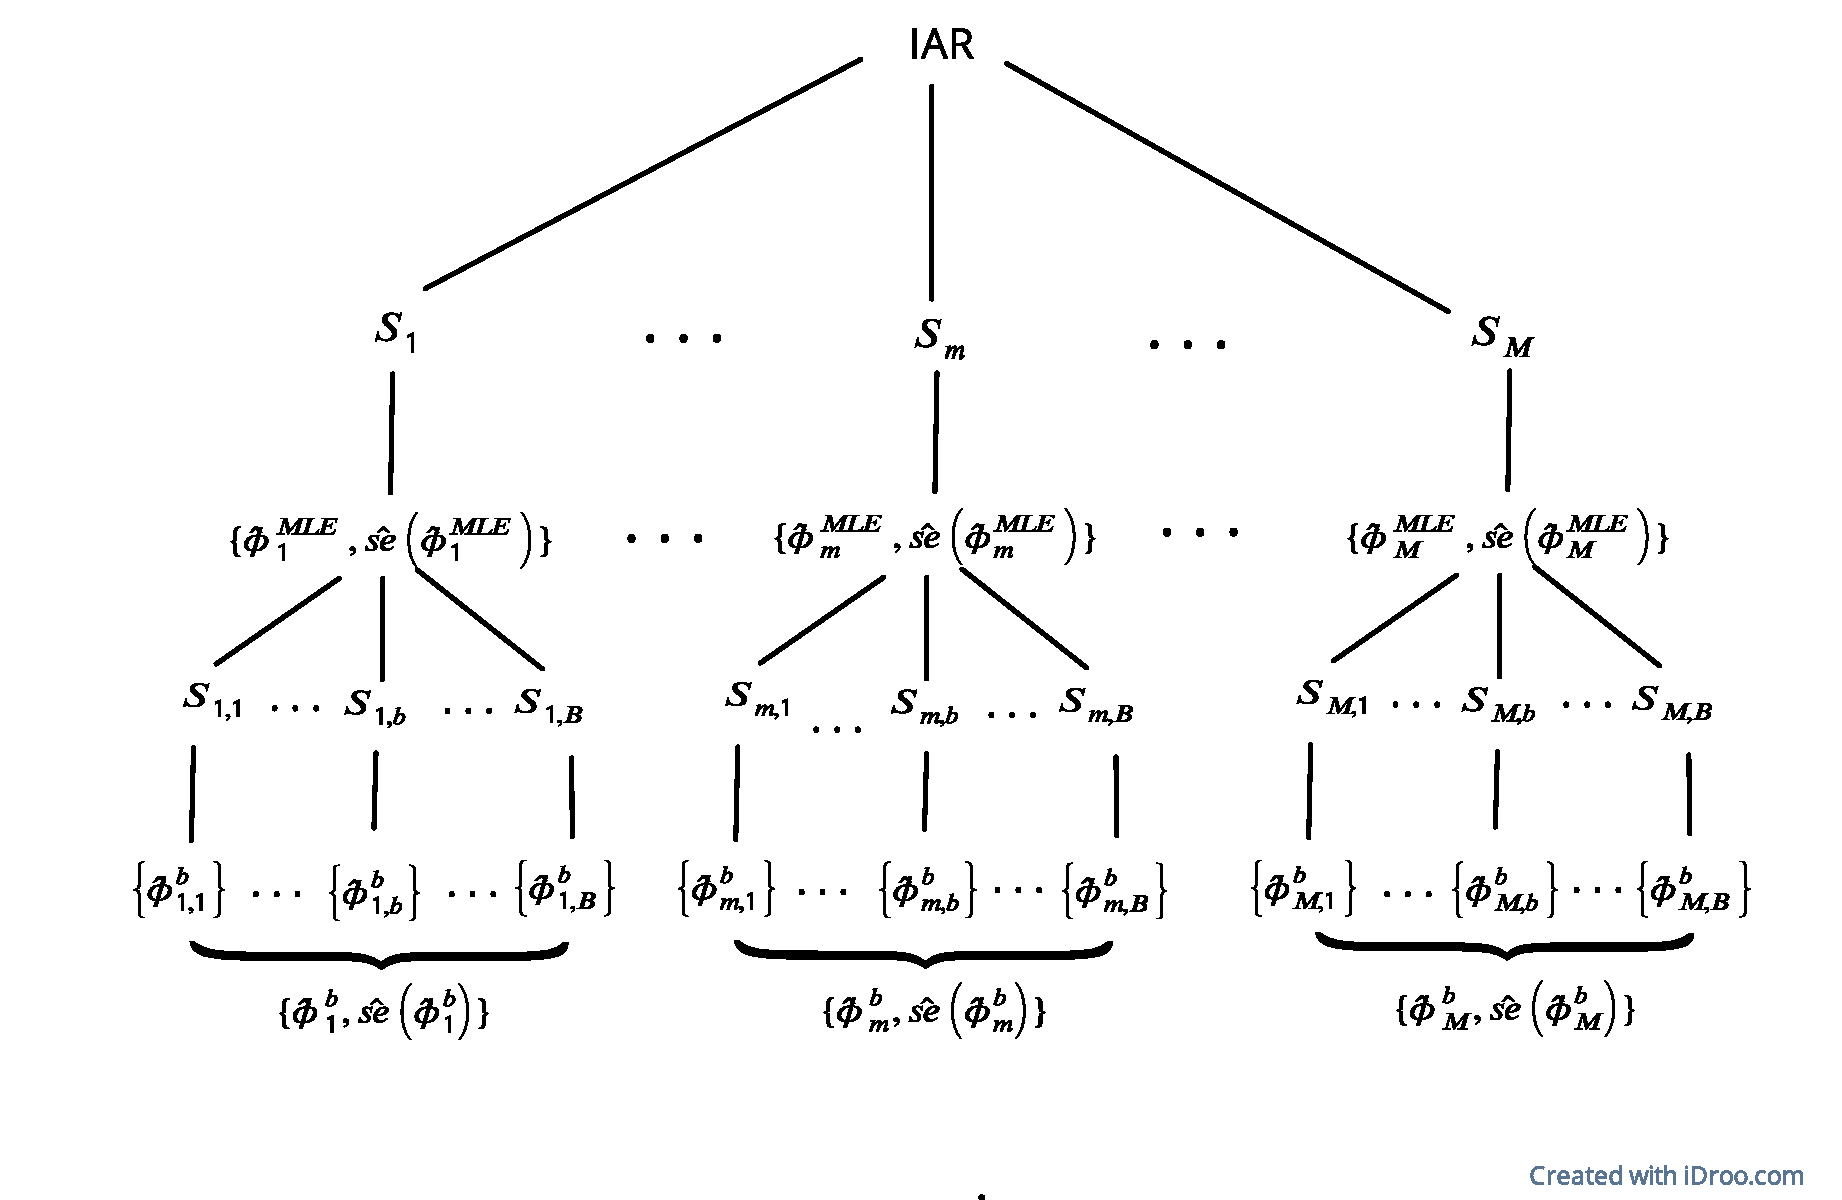
\includegraphics[trim={0 2cm 0 0},clip,width=0.9\textwidth]{Kap3/Fig_Cap3/4RzQZ8xYXY.pdf}
    \caption{Esquema general del estudio de Monte Carlo.}
    \label{fig:monte_carlo1}
\end{figure}

En este estudio, se evaluaron los resultados del modelo en el caso de tiempo irregularmente espaciado, aunque también se comprobó que el modelo es válido para tiempos regulares con $\Delta_n=1$ para todos los valores de $n$.

Para analizar el comportamiento de los estimadores de máxima verosimilitud y bootstrap, 
se realizaron simulaciones de distribuciones de muestras finitas.
Los resultados de estas simulaciones se muestran en las figuras \ref{fig:monte_carlo_res1} y \ref{fig:monte_carlo_res2}. 
Se puede observar que ambos estimadores presentan un comportamiento satisfactorio, parecen ser insesgados y consistentes en sus resultados.

\begin{figure}[h]
    \begin{minipage}{0.45\textwidth}
    \includegraphics[width=0.8\linewidth,angle = 270]{Kap3/Fig_Cap3/sim3.eps}
    \caption{Esquema general del estudio de Monte Carlo.}
    \label{fig:monte_carlo_res1}
    \end{minipage}
    \hfill
    \begin{minipage}{0.45\textwidth}
    \includegraphics[width=0.8\linewidth,angle = 270]{Kap3/Fig_Cap3/sim4.eps}
    \caption{Esquema general del estudio de Monte Carlo.}
    \label{fig:monte_carlo_res2}
    \end{minipage}
\end{figure}

Note que para valores pequeños de $n$ y para valores cercanos a cero de $\phi$, 
los estimadores tienden a tener una mayor variabilidad.
Este hallazgo es importante para el análisis de los resultados, 
ya que sugiere que la precisión de los estimadores puede verse afectada por factores como la cantidad de datos 
disponibles y la magnitud del parámetro de interés.

% \begin{figure}[h]
%     \centering
%     \subfigure[Estimación por Máxima verosimilitud]{
%       \includegraphics[width=0.5\textwidth, angle = 270]{Kap3/Fig_Cap3/sim3.eps}
%       \label{fig:monte_carlo_res1}
%     }
%     \subfigure[Estimación por Bootstrap]{
%       \includegraphics[width=0.5\textwidth, angle = 270]{Kap3/Fig_Cap3/sim4.eps}
%       \label{fig:monte_carlo_res2}
%     }
%     \caption{Resultados de la distribución de muestras finitas simuladas. (a) contiene las estimaciones por
%     máxima verosimilitud y (b) contiene los resultados de la estimación por Bootstrap }
%     \label{fig:monte_carlo}
%   \end{figure}

En segundo lugar, para ambos estimadores, presentamos las medidas de rendimiento. Por separado, estimamos el error de Monte Carlo (MCE) por teoría asintótica cada simulación (véase, Koehler et al., 2009), y luego presentamos el valor máximo.
 askjdikas


 
